\documentclass[kursovay]{nanolab}

\usepackage{multirow}
\usepackage{array}
\usepackage[hidelinks]{hyperref}

% \includeonly{parts/original, parts/review}

\renewcommand{\phi}{\varphi}
\renewcommand{\Phi}{\varPhi}
\renewcommand{\Theta}{\varTheta}
\newcommand{\unchapter}[1]{%
  \begingroup
  \chapter*{#1}
  \addcontentsline{toc}{chapter}{\textbf{#1}}
  \markboth{#1}{}
  \endgroup
}

\hyphenation{уп-рав-ле-ния}
\hyphenation{ус-тройств}
\hyphenation{ме-та-по-вер-хно-сти}

\extrarowheight=3pt

\begin{document}

\begin{titlepage}
    %\begin{centering}
    {\Large \center
        МОСКОВСКИЙ ГОСУДАРСТВЕННЫЙ УНИВЕРСИТЕТ

        имени М.В. ЛОМОНОСОВА

        ФИЗИЧЕСКИЙ ФАКУЛЬТЕТ

        Кафедра нанофотоники

    }
    \begin{centering}
        \vspace{4cm}
        \Large
        \centering
        Когерентный контроль распространения света с помощью микродифракционных решёток\\
    \end{centering}
    \vspace{4cm}
    \begin{flushright}
        \underline{курсовая работа}

        студента 204 группы

        Нецветаева~А.~А. \vspace{1.5cm}

        \underline{научный руководитель}:

        м.н.с. Фролов~А.~Ю.

    \end{flushright}
    \vspace{4cm}
    \begin{centering}
        Москва --- 2024

    \end{centering}
\end{titlepage}

\tableofcontents
\chapter*{Введение}

Способность контролировать и направлять оптические лучи имеет решающее значение для новых технологий. Среди них — лидар (англ. LiDAR, Light Detection and Ranging, «обнаружение и определение дальности с помощью света»)\cite{jaboyedoff2012use}, лазерная визуализация\cite{holmstrom2014mems}, атмосферная оптическая линия связи (АОЛС)\cite{khalighi2014survey} и однопиксельная визуализация\cite{edgar2019principles}.
\chapter*{Обзор литературы}

\section{Когерентный контроль}

Метод когерентного контроля в общем случае заключается в изучении зависимости интерференционной картины, полученной после взаимодействия двух когерентных пучков, распространяющихся в противоположных направлениях, с оптически неоднородной средой (структурой), от разности фаз этих пучков. При таком взаимодействии в пространстве образуется стоячая электромагнитная волна, и степень влияния неоднородности на интерференционную картину определяется положениями пучностей и узлов относительно структуры. При рассмотрении сред, линейные размеры которых по направлению распространения излучения (толщина) значительно меньше длины волны, можно выделить два предельных случая:
\begin{enumerate}
    \item Когерентное полное пропускание (CPT, англ. ``coherent perfect transmission''). Структура находится в узле стоячей волны. Тогда неоднородность становится <<выключенной>> и практически не влияет на распространение излучения.
    \item Когерентное полное поглощение (CPA, англ. ``coherent perfect absorption''). Структура находится в пучности. Тогда влияние неоднородности максимально.
\end{enumerate}
За счёт этих двух состояний можно реализовывать полностью оптическое переключение, а рассмотрев другие предельные случаи, даже реализовать базовые логические операции (Рис. \ref{fig:opticalLogic})\cite{twoDimensional2016}. Также когерентный контроль позволяет модулировать интенсивность в широких пределах\cite{lightWithLight2012}, создавать оптические транзисторы\cite{lightWithLight2015}, измерять поглощение и другие характеристики материалов неразрушающим путем\cite{CPAGraphene2017} и многое другое.

\begin{figure}
    \begin{center}
        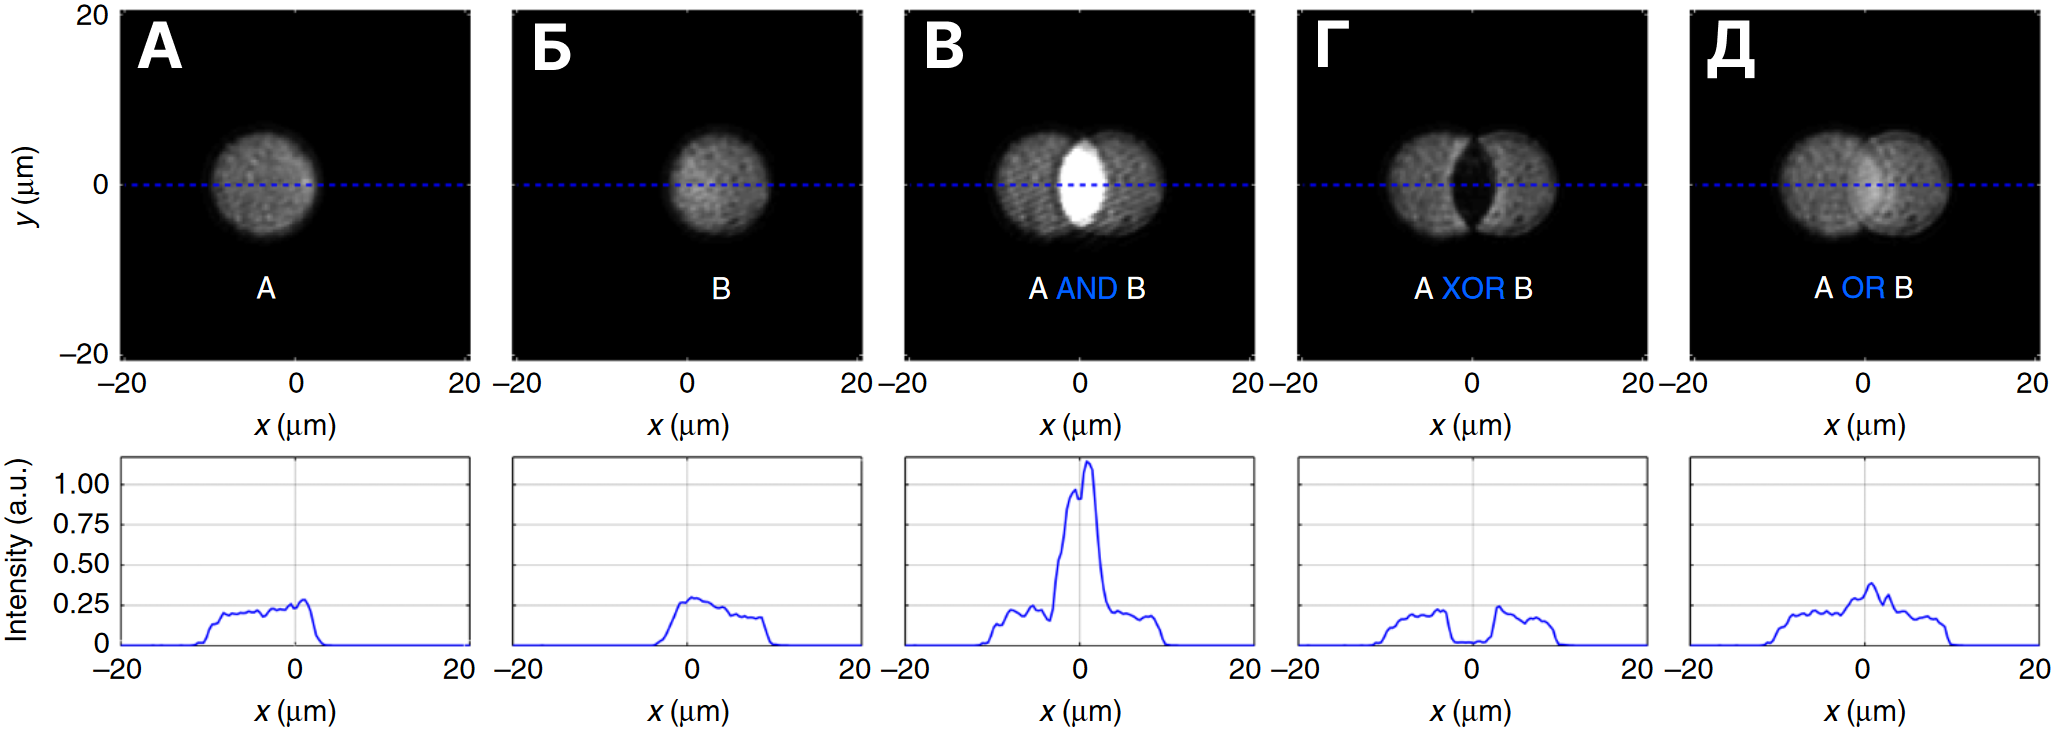
\includegraphics[width=\textwidth]{pictures/Optical_logic.png}
        \caption{Оптические базовые логические операции. Изображения метаповерхности, \textbf{(А)} освещенной только лучом $A$, \textbf{(Б)} только лучом $B$ и \textbf{(В-Д)} обоими лучами $A$ и $B$. Разным относительным фазам лучей $A$ и $B$ соответствуют разные логические операции: \textbf{(В)} $A$ И $B$ ($\Theta = \pi$), \textbf{(Г)} $A$ <<ИСКЛЮЧАЮЩЕЕ ИЛИ>> $B$ ($\Theta = 0$) и \textbf{(Д)} $A$ ИЛИ $B$ ($\Theta = \pm \pi/3$). На графиках показан профиль интенсивности вдоль соответствующей пунктирной синей линии. Уровни интенсивности показаны в одинаковых оттенках серого на всех изображениях и в одном вертикальном масштабе на всех графиках.\cite[Fig. 3]{twoDimensional2016}}
    \end{center}
    \label{fig:opticalLogic}
\end{figure}

Теоретически метод когерентного контроля можно описать с помощью комплексной матрицы рассеяния. Пусть два когерентных оптических пучка $E_\alpha$ и $E_\beta$, распространяющихся в противоположных направлениях, падают по нормали на некоторый слой материала с линейными оптическими характеристиками и пусть при взаимодействии с материалом сохраняется поляризация излучения. Две результирующие волны (по обе стороны от плоскости материала) обозначим $E_\delta$ и $E_\gamma$. Тогда соответствующие напряженности электрических полей связаны матрицей рассеяния $\matr{S}$:
\begin{equation}
    \begin{bmatrix}
        E_\delta \\
        E_\gamma
    \end{bmatrix} = \begin{bmatrix}
        S_{11} & S_{12} \\
        S_{21} & S_{22}
    \end{bmatrix} \begin{bmatrix}
        E_\alpha \\
        E_\beta
    \end{bmatrix}.  
    \label{scatteringMatrix}
\end{equation}
Аналитические выражения для коэффициентов $S_{ij}$, которые зависят от характеристик материала, приводятся в \cite{CPATheory2015}.

\section{Обобщенный закон Снелла}

Пусть каждой точке $M(x)$ границы раздела соответствует значение фазы, равное $\Phi(x)$ и пусть падающая на границу раздела волна, проходящая через заданную точку $M(x)$, претерпевает фазовый разрыв $\Phi(x)$. Для такой границы мы вынуждены пересмотреть классический закон Снелла, описываемый формулой
\begin{equation}
    n_i \sin \Theta_i = n_t \sin \Theta_t
\end{equation}
в соответствии с принципом Ферма.

Рассмотрим плоскую волну, падающую под углом $\Theta_i$ . Если предположить, что два пути бесконечно близки к реальному пути света (Рис. \ref{fig:generalized}А), то разность фаз между ними равна нулю
\begin{equation}
    \label{eq:opticalPathLengthDifference}
    [k_0n_i\sin\Theta_i\, dx + (\Phi + d\Phi)] - [k_0n_t\sin\Theta_t\,dx + \Phi] = 0,
\end{equation}
где $\Theta_t$ --- угол преломления; $\Phi$ и $\Phi + d\Phi$ --- разрывы фаз в местах пересечения границы раздела синим и красным путями соответственно; $dx$ --- расстояние между точками пересечения; $n_i$ и $n_t$ --- показатели преломления двух сред; $k_0 = 2\pi/\lambda_0$ --- волновое число, где $\lambda_0$ --- длина волны в вакууме. Если градиент фазы $d\Phi/dx$ создан постоянным, предыдущее уравнение \eqref{eq:opticalPathLengthDifference} приводит к обобщенному закону преломления Снелла
\begin{equation}
    \label{eq:generalizedRefraction}
    n_t\sin\Theta_t - n_i \sin\Theta_i = \frac{\lambda_0}{2\pi}\frac{d\Phi}{dx}.
\end{equation}

Уравнение \eqref{eq:generalizedRefraction} показывает, что преломленный луч может иметь произвольное направление при условии, что создан подходящий постоянный градиент фазы $d\Phi/dx$ вдоль границы раздела (Рис.~\ref{fig:generalized}Б) \cite{generalized2011}. Более того, при ненулевом градиенте фазы два угла падения $\pm \Theta_i$ соответствуют различным углам преломления. Как следствие, существуют два угла полного внутреннего отражения
\begin{equation}
    \Theta_c = \arcsin \left(\pm\frac{n_t}{n_i} - \frac{\lambda_0}{2\pi}\frac{d\Phi}{dx}\right)
\end{equation}

Аналогично, для отражения имеем
\begin{equation}
    \label{eq:generalizedReflection}
    \sin\Theta_r - \sin\Theta_i = \frac{\lambda_0}{2\pi n_i}\frac{d\Phi}{dx},
\end{equation}
где $\Theta_r$ --- угол отражения. Между $\Theta_r$ и $\Theta_i$ существует нелинейная связь, которая заметно отличается от известного закона геометрической оптики. Уравнение \eqref{eq:generalizedReflection} показывает, что всегда существует критический угол падения
\begin{equation}
    \Theta_c' = \arcsin\left(1 - \frac{\lambda_0}{2\pi n_i}\left|\frac{d\Phi}{dx}\right|\right),
\end{equation}
при котором отраженная волна становится эванесцентной.

Обобщенный закон Снелла открывает широкие возможности для управления распространением света.

\begin{figure}
    \begin{center}
        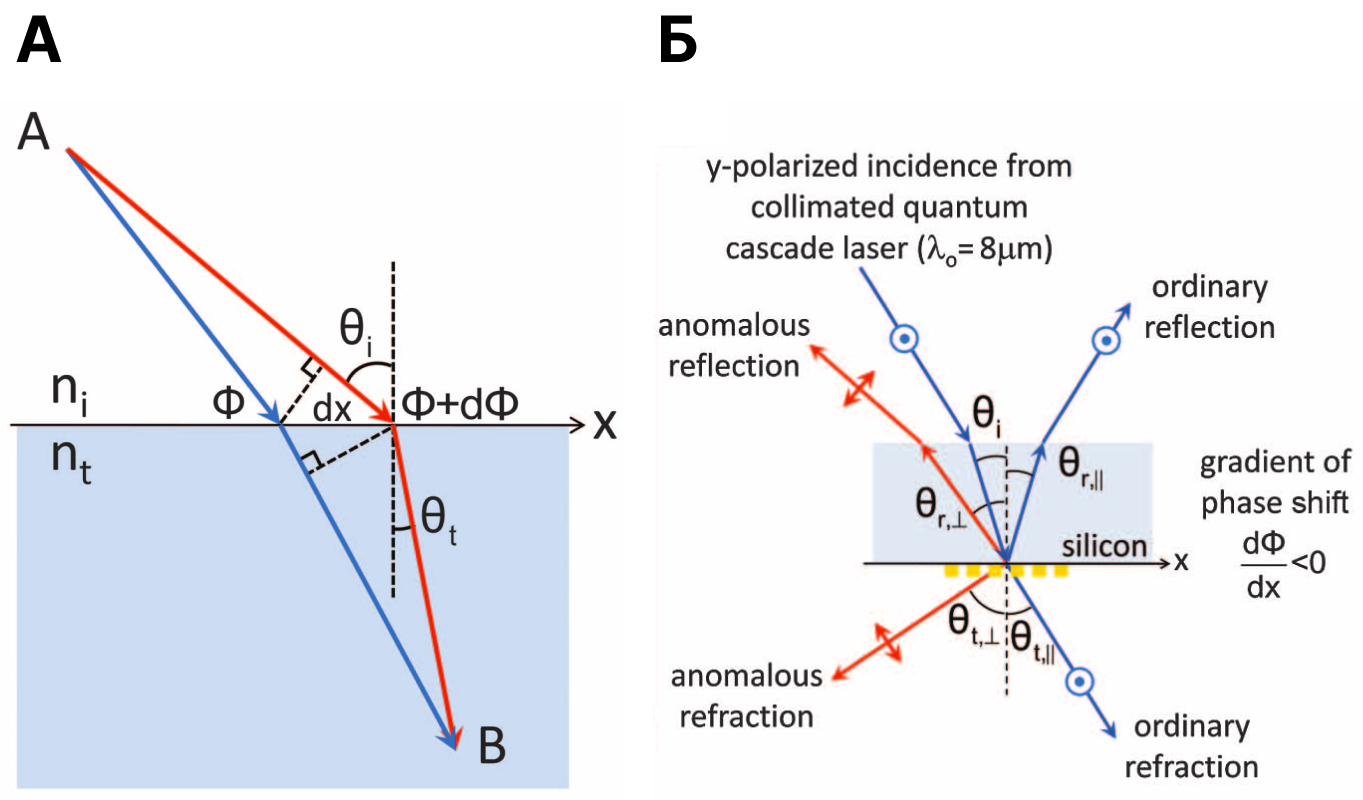
\includegraphics[width=0.92\textwidth]{pictures/Generalized_Snell's_law.png}
        \caption{\textbf{(А)} Рисунок, используемый для вывода обобщенного закона преломления Снелла. Граница между двумя средами искусственно структурирована так, чтобы внести резкий фазовый сдвиг на пути света, который зависит от положения на границе раздела. $\Phi$ и $\Phi + d\Phi$ — фазовые сдвиги, при которых два луча (синий и красный) пересекают границу.\cite[Fig. 1]{generalized2011} \textbf{(Б)} Схема экспериментальной установки, демонстрирующей обобщенный закон Снелла.\cite[Fig. 3B]{generalized2011}}
    \end{center}
    \label{fig:generalized}
\end{figure}

\section{Управление распространением света}
Способность направлять оптические лучи имеет решающее значение для современных технологий. Среди них — лидар (англ. LiDAR, Light Detection and Ranging, «обнаружение и определение дальности с помощью света»)\cite{jaboyedoff2012use}, лазерная визуализация\cite{holmstrom2014mems}, атмосферная оптическая линия связи (АОЛС)\cite{khalighi2014survey} и однопиксельная визуализация\cite{edgar2019principles}. Ранние методы предполагали механическое и электрическое управление оптическими элементами: повороты и перемещения зеркал и линз, изменение показателя преломления жидкого кристалла под действием приложенного напряжения и т. д.\cite{tholl2006novel}. Однако такие устройства были громоздкими и ограниченными в скорости и надежности. Развитие технологий изготовления структур нанометровых масштабов и успехи в исследовании взаимодействия света с ними позволяют создавать более эффективные и производительные полностью оптические системы.

\paragraph*{Характеристики способов управления.}
Для достижения параметров, необходимых для реальных приложений, системы управления должны обладать определенными характеристиками. А именно, пучок должен быть достаточно узким и подчиняться управлению в большом диапазоне углов, называемом полем зрения (FOV, field of view): вплоть до 180$^\circ$ для одномерного сканирования и до полусферы для двухмерного сканирования. Кроме того, угол излучения должен перенастраиваться в реальном времени на высокой скорости с минимальными потерями интенсивности. В настоящее время существует несколько способов управления пучком, основанных на методе когерентного контроля: активные метаповерхности, медленное световое сканирование и оптические фазовые антенные решетки (ФАР). Рассмотрим их подробнее.

% Диаграмма направленности (ДН) $F (\vec \xi\,)$ устройства управления пучком может быть определена из его ближнего электромагнитного поля $E(\vec r\,)$ с помощью преобразования Фурье:
% \begin{equation}
%     \label{eq:Fourier}
%     F(\vec \xi\,) = \iint E(\vec r\,)\, e^{ik_0\left(\vec r \cdot \vec \xi\,\right)}\, d^2\vec r,
% \end{equation}
% где вектор $\vec \xi = (\phi, \Theta)$ показывает полярное и азимутальное направления, \mbox{$\vec r = (x, y)$} указывает на точку на активной поверхности, $k_0$ --- волновое число.

% По характеру \eqref{eq:Fourier}, можно видеть, что модулирование ближнего поля $E(\vec r\,)$ плоской волной $e^{ik_0\,\vec r \cdot \vec k}$ соответствует сдвигу ДН на вектор $\vec k$. Таким образом, пик, изначально находящийся в начале координат может быть перемещен на произвольный угол. В этом заключается основа оптического управления распространением света

\paragraph*{Метаповерхности.}
Метаповерхности представляют собой структуры субволновых оптических элементов --- антенн, реализующих пространственно изменяющийся фазовый разрыв для падающей плоской волны. Градиент фазы взаимодействующего света определяется геометрией антенн и характеристиками материала изготовления метаповерхности. В соответствии с обобщенным законом Снелла, за счёт наличия градиента фазы наблюдается как нормальный прошедший пучок, так и аномальный (Рис. \ref{fig:metasurfaces}А), отклоняющийся на угол, определяемый \eqref{eq:generalizedReflection}. Так, в работе\cite{huang2016gate} экспериментально осуществлялась <<перекачка>> интенсивности между нулевым и $\pm1$ порядками дифракции, распространяющихся под углом $40^\circ$ к нормали\cite{huang2016gate}.

\paragraph*{Медленное световое сканирование.}

\begin{figure}
    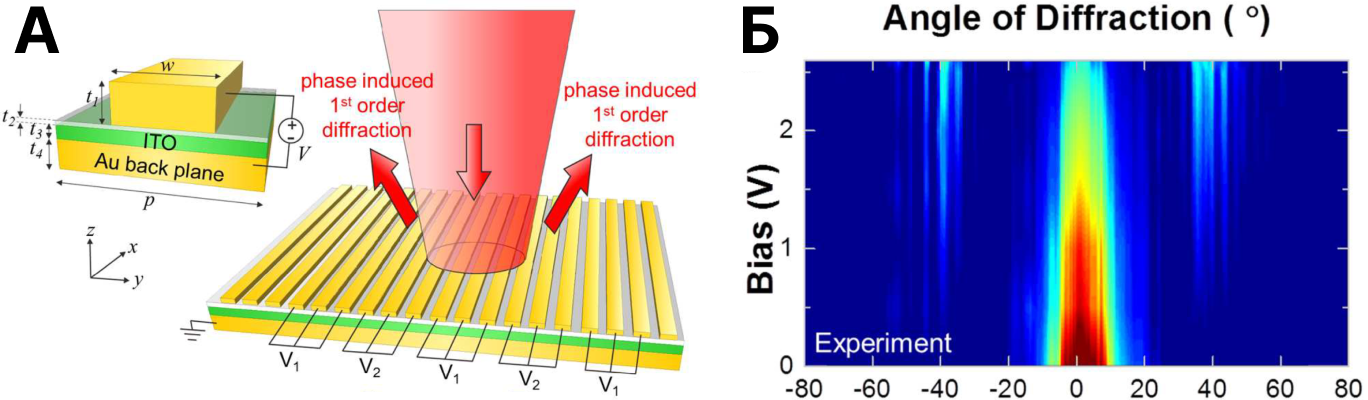
\includegraphics[width=\textwidth]{pictures/Metasurfaces.png}
    \caption{\textbf{(А)} \cite[Fig. 1A]{huang2016gate} \textbf{(Б)} \cite[Fig. 4B]{huang2016gate}}
    \label{fig:metasurfaces}
\end{figure}
\chapter{Оригинальные результаты}

\section{Численное моделирование дифракционной решетки с переменным периодом.}

\subsection{Исследуемый образец}
В качестве исследуемой оптически неоднородной среды для метода когерентного контроля была выбрана дифракционная решетка в виду относительной простоты изготовления и изучения. Для непрерывного управления направлением распространения пучка была разработана трапециевидная форма щелей, такая, что при изменении относительной фазы двух когерентных источников эффективный период решетки непрерывно меняется за счёт сдвига пучности результирующей стоячей волны. В качестве материала был выбран аморфный кремний за его большой показатель преломления $n = 3,48$ и практически нулевой коэффициент поглощения для исследуемой длины волны $\lambda = 1550\ \text{нм}$. Для расчетов использовались табличные характеристики кремния, представленные на сайте\cite{refractiveIndex}. Полученная структура имеет множество геометрических параметров, а именно: периоды решетки и длины оснований трапеций на верхней и нижней границах $d_t$, $b_t$, $d_b$ и $b_b$ соответственно ($d_t < d_b$), число периодов $N$ и высота структуры $h$, указанные на Рис. \ref{fig:structure}А.

\begin{figure}
    \begin{center}
        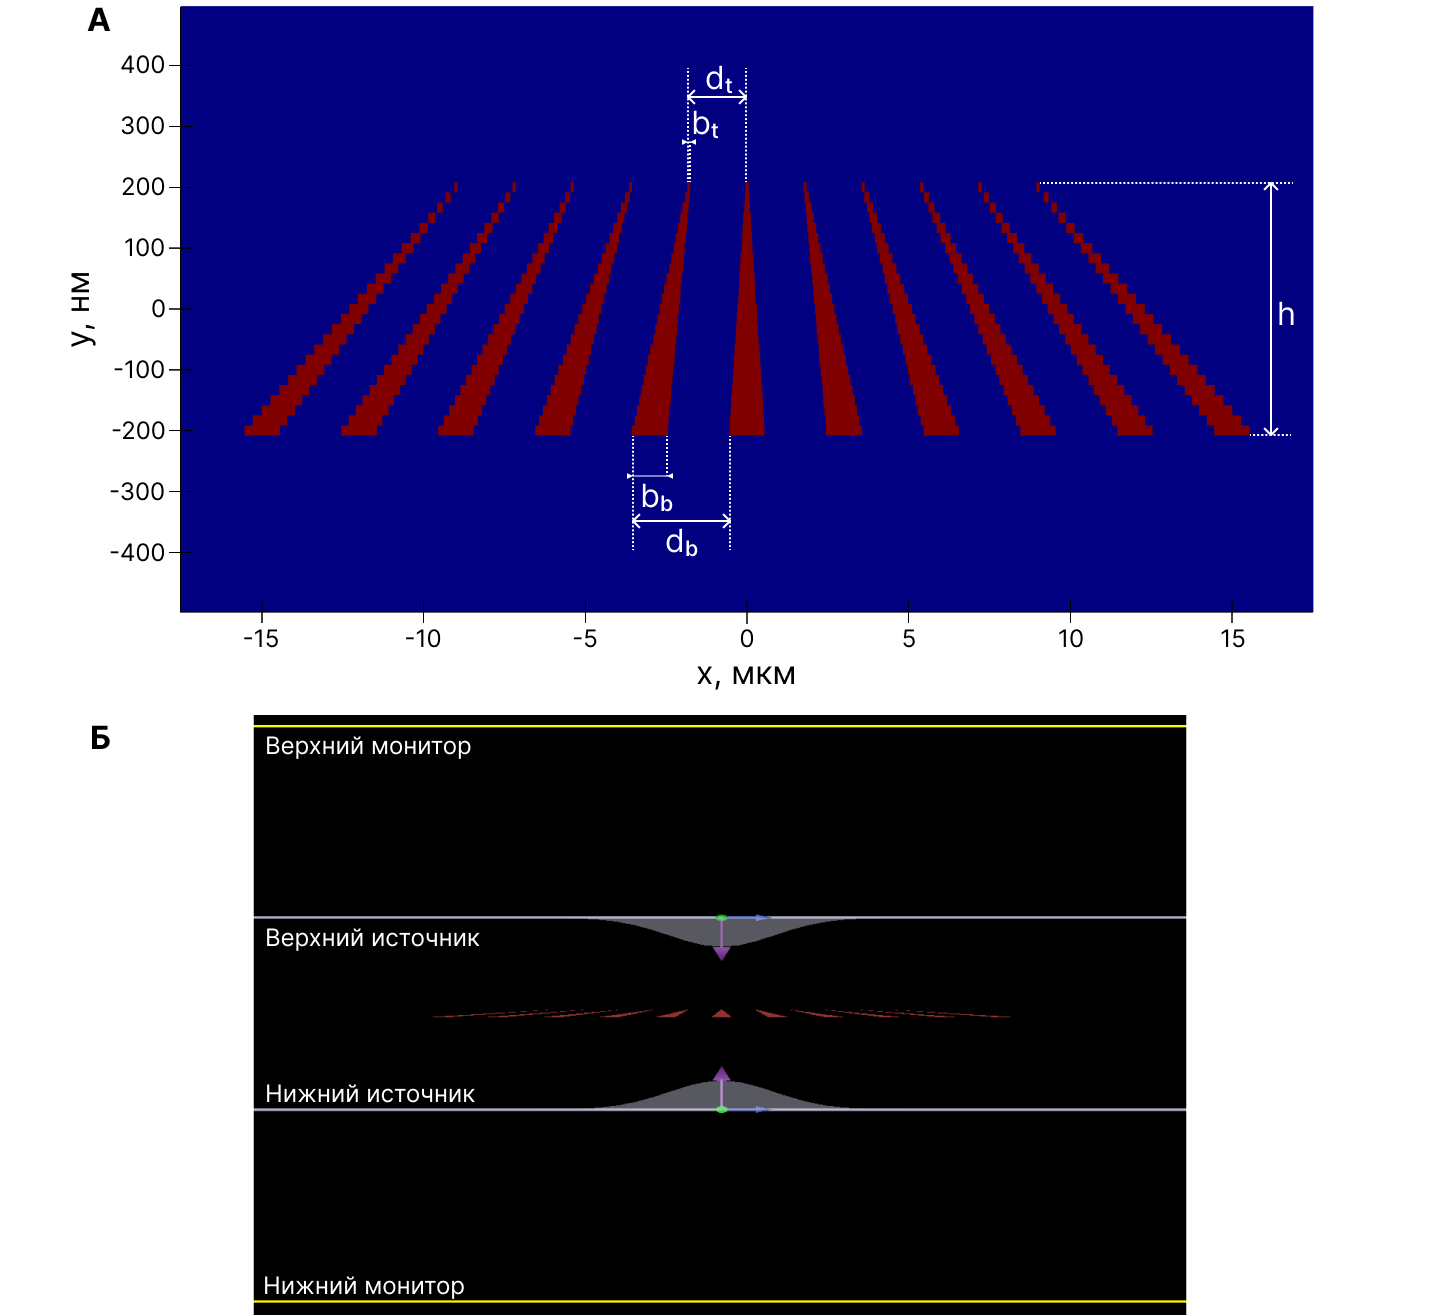
\includegraphics[width=\textwidth]{pictures/Structure.png}
        \caption{\textbf{(А)} Визуализация показателя преломления структуры с помощью монитора, представленного в пакете \texttt{Lumerical}. Параметры на рисунке: $d_t = 1800\ \text{нм}$, \mbox{$b_t = 300\ \text{нм }$}, $d_b = 3000\ \text{нм}$, $b_b = 1000\ \text{нм}$, $N = 11$, $h = 400\ \text{нм}$. Наблюдаемая <<лесенка>> связана с внутренним представлением области FDTD в программе. \textbf{(Б)}~Схема моделируемой системы.}
        \label{fig:structure}
    \end{center}
\end{figure}

\subsection{Программное обеспечение}
Основные результаты данной работы получены при помощи программного пакета \texttt{Ansys Lumerical FDTD} версии \texttt{2024 R1}, позволяющего моделировать поведение различных оптических систем. Его работа основана на численном методе конечных разностей во временной области (FDTD, англ. <<finite-difference time-domain>>). Характерные графики были построены на языке \texttt{Python} с помощью библиотек \texttt{numpy} и \texttt{matplotlib}. Результаты были структурированы и наглядно представлены с применением веб-технологий на языке \texttt{JavaScript}.

\subsection{Моделируемая система}
Схема моделируемой системы приведена на Рис. \ref{fig:structure}Б. На одинаковых расстояниях от структуры были расположены когерентные гауссовы источники с длиной волны $1550\ \text{нм}$ и длительностью импульса $10\ \text{фс}$. За ними находятся мониторы, которые выполняют Фурье-преобразование электрического поля и показывают профиль интенсивности дальнего поля. Радиус перетяжки $w = 5\ \text{мкм}$ был выбран так, чтобы задействовать максимальное число периодов решетки, но чтобы при этом дифракция на краях структуры была незначительной. Число периодов $10 \leqslant N \leqslant 15$ было ограничено из практических соображений сложности изготовления более протяженной решетки. Толщина $h \approx \lambda/4$ примерно равнялась четверти длины волны, чтобы на структуре при заданной разности фаз находилась только одна пучность, то есть имелся единственный эффективный период.

Время симуляции подбиралось таким образом, чтобы уровень энергии в системе к моменту окончания расчетов был достаточно низким, иначе полученные результаты могли бы оказаться неточными. Использовались граничные условия типа PML (англ. <<perfectly matched layer>>, <<идеально поглощающие слои>>), которые представляют собой поглощающую границу, моделирующую уход волны на бесконечность. Тем не менее, какая-то часть волн может отражаться от стенок и попадать обратно в область симуляции, приводя к искажениям. Шаг сетки, на которой программа выполняла численные расчеты, подбирался исходя из компромисса между временем симуляции и достаточным разрешением представления структуры.

\section{Расчет зависимости интенсивности излучения в первом дифракционном порядке от угла дифракции и сдвига фаз между источниками}

Исходя из качественных соображений и простейшего уравнения дифракционной решетки для нормального падения пучка:
\begin{equation}
    d\sin\Theta_m = m\lambda,
    \label{eq:simpleGrating}
\end{equation}
были ограничены $d_t$ и $d_b$ решетки так, чтобы наблюдался только первый порядок дифракции:
\begin{equation}
    d_{min} = \lambda = 1550\ \text{нм},\ d_{max} = 2\lambda = 3100\ \text{нм}.
\end{equation}
Приблизительно в данных пределах фиксировались определенные значения $d_t$ и $d_b$, связанные с углом обзора соотношением
\begin{equation}
    \mathrm{FOV} = \Theta_{max} - \Theta_{min} = \arcsin{\frac{\lambda}{d_t}} - \arcsin{\frac{\lambda}{d_b}},
    \label{eq:fov}
\end{equation}
и циклично запускалась симуляция, на каждом шаге которой последовательно изменялись $b_t$ и $b_b$ в пределах 100--1500 нм и сохранялись результаты вычислений с обоих мониторов. Таким образом, для каждой пары $d_t$--$d_b$ было получено \mbox{$15 \cdot 15 \cdot 2 = 450$} наборов данных, по которым затем строились графики зависимости интенсивности излучения в первом дифракционном порядке от угла дифракции и сдвига фаз между источниками типа <<тепловая карта>>.

\begin{figure}
    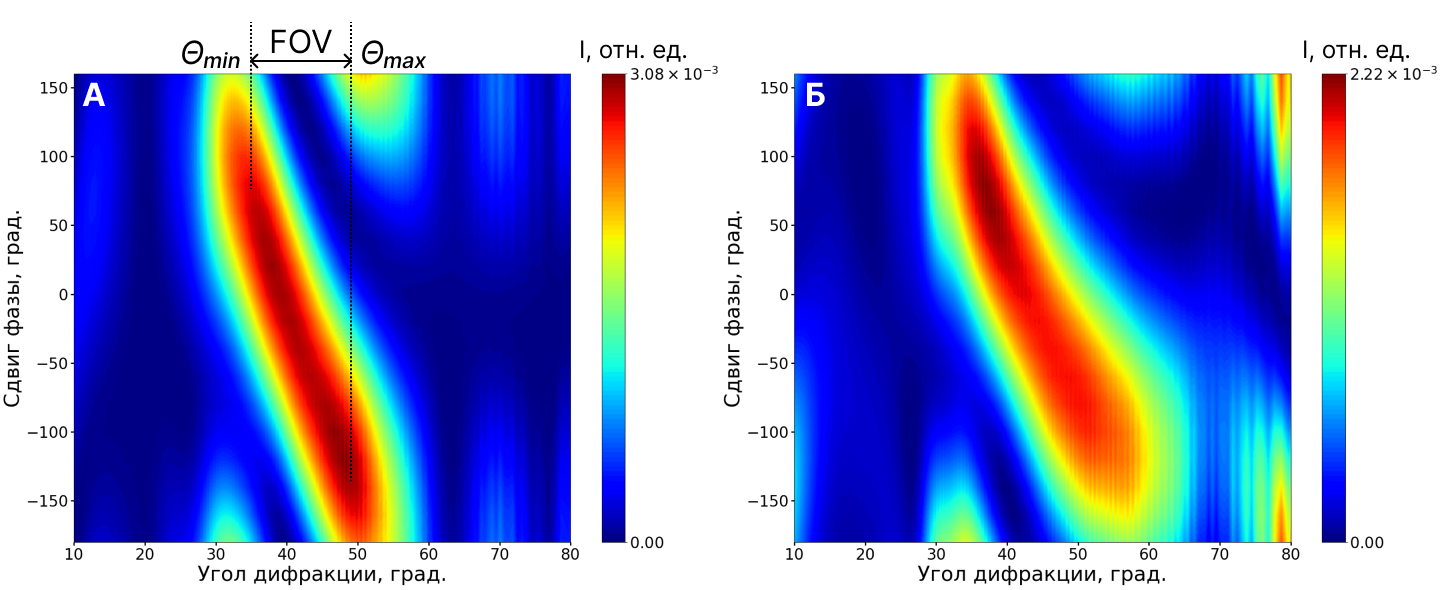
\includegraphics[width=\textwidth]{pictures/Heatmaps.png}
    \caption{Избранные графики зависимости интенсивности излучения в первом дифракционном порядке от угла дифракции и сдвига фаз между источниками. \textbf{(А)} Полученная конфигурация с углом обзора 15°: $N = 11$, $d_t = 1800$~нм, $d_b = 3000$~нм, $b_t = 1100$~нм, $b_b = 500$~нм. \textbf{(Б)} Полученная конфигурация с углом обзора 20°: $N = 15$, $d_t = 1550$~нм, $d_b = 3100$~нм, $b_t = 1100$~нм, $b_b = 400$~нм. }
\end{figure}

\section{Результаты}

Все полученные графики представлены на \href{https://fizfakovets.github.io}{\underline{сайте}}. Были найдены конфигурации, позволяющие осуществлять непрерывный контроль распространения пучка в диапазоне 35--55°. В результате оптимизации значений $b_t$ и $b_b$ удалось достичь равномерной интенсивности дифракционного порядка при изменении фазы одного из источников. В рамки настоящей работы не входило достижение высокого разрешения сканирования, поэтому на графике можно видеть большую угловую расходимость пучка. Однако это можно исправить, направляя на решетку более коллимированное излучение.

\chapter*{Заключение}

Заключение
\bibliographystyle{unsrt}
\bibliography{refs}

\end{document}